              %******************************************%
              %                                          %
              % Modello di tesi di laurea o di dottorato %
              %            di Lorenzo Pantieri           %
              %                                          %
              %                © 2013-2017               %
              %                                          %
              %******************************************%
       

% I seguenti commenti speciali impostano:
% 1. utf8 come codifica di input,
% 2. PDFLaTeX come motore di composizione;
% 3. Tesi.tex come documento principale;
% 4. il controllo ortografico italiano per l'editor.

% !TEX encoding = UTF-8 Unicode
% !TEX TS-program = pdflatex
% !TEX root = Tesi.tex
% !TEX spellcheck = it-IT

\documentclass[11pt,%                      % corpo del font principale
               a4paper,%                   % carta A4
               twoside,openright,%         % fronte-retro
%              oneside,openany,%           % solo fronte
               titlepage,%                 % frontespizio
               headinclude,,footinclude,%  % testatina e piede di pagina
               BCOR5mm,%                   % rilegatura di 5 mm
               cleardoublepage=empty,%     % pagine vuote senza testatina e piede di pagina
               captions=tableheading,%     % didascalie in cima alle tabelle
               ]{scrreprt}                 % classe report di KOMA-Script;
               
\usepackage[T1]{fontenc}                   % codifica dei font:
                                           % NOTA BENE! richiede una distribuzione *completa* di LaTeX,
                                           % per esempio TeXLive o MiKTeX *complete*

\usepackage[utf8]{inputenc}                % codifica di input; anche [latin1] va bene
                                           % NOTA BENE! va accordata con le preferenze dell'editor

\usepackage[english,italian]{babel}        % per scrivere in italiano e in inglese;
                                           % l'ultima lingua (l'italiano) risulta predefinita

\usepackage[suftesi]{frontespizio}         % frontespizo
                                           % per includerlo nel documento bisogna:
                                           % 1. compilare una prima volta Tesi.tex;
                                           % 2. compilare a parte Tesi-frn.tex, generato dalla compilazione precedente;
                                           % 3. compilare ancora Tesi.tex. 

\usepackage{indentfirst}                   % rientra il primo capoverso di ogni sezione

\usepackage{graphicx}                      % immagini

\usepackage{listings}                      % codici

\usepackage[font=small]{quoting}           % citazioni

\usepackage{amsmath,amssymb,amsthm}        % matematica

\usepackage[italian]{varioref}             % riferimenti completi della pagina

\usepackage{tabularx}                      % tabelle di larghezza prefissata

\usepackage[autostyle,italian=guillemets]{csquotes} % virgolette ottimizzate per biblatex

\usepackage[style=philosophy-modern,hyperref,square,backend=biber]{biblatex}
                                           % eccellente pacchetto per la bibliografia;
                                           % produce uno stile di citazione autore-anno; 
                                           % lo stile "numeric-comp" produce riferimenti numerici;
                                           % NOTA BENE! bisogna che il proprio editor sia configurato per biber
                                          
\addbibresource{Bibliografia.bib}          % database di biblatex 
                                          
\usepackage{subfig}                        % sottofigure, sottotabelle

\usepackage{lipsum}                        % testo fittizio

\usepackage{eurosym}                       % simbolo dell'euro

\usepackage[eulerchapternumbers,%          % numeri dei capitoli nel font Euler
            subfig,%                       % se si usa il pacchetto subfig
            beramono,%                     % Bera Mono come font a spaziatura fissa
            eulermath,%                    % AMS Euler come font per la matematica
            pdfspacing,%                   % migliora il riempimento di riga
            listings,%                     % codici
%           parts,%                        % da decommentare in un documento diviso in parti
            ]{classicthesis}               % stile ClassicThesis

\usepackage{arsclassica}                   % modifica l'aspetto di ClassicThesis

%*********************************************************************************
% impostazioni-tesi.tex
% di Lorenzo Pantieri (2013-2016)
% file che contiene le impostazioni della tesi
%*********************************************************************************


%*********************************************************************************
% Comandi personali
%*******************************************************
\newcommand{\myName}{Marco De Martino}                           % autore
\newcommand{\myTitle}{appunti sul marmo} % titolo
\newcommand{\myDegree}{Tesi di laurea}                           % tipo di tesi
\newcommand{\myUni}{Conservatorio di Musica S. Cecilia di Roma}       % universit�
\newcommand{\myFaculty}{Musica Elettronica}        % facolt\'a
\newcommand{\myDepartment}{Nuove Tecnologie}             % dipartimento
\newcommand{\myProf}{Prof.~Michelangelo Lupone}          % relatore
\newcommand{\myOtherProf}{Prof.~Nicola Bernardini}                  % correlatore (se presente)
\newcommand{\myLocation}{Roma}                                 % dove
\newcommand{\myTime}{Aprile 2017}                               % quando



%*********************************************************************************
% Impostazioni di amsmath, amssymb, amsthm
%*********************************************************************************

% comandi per gli insiemi numerici (serve il pacchetto amssymb)
\newcommand{\numberset}{\mathbb} 
\newcommand{\N}{\numberset{N}} 
\newcommand{\R}{\numberset{R}} 

% un ambiente per i sistemi
\newenvironment{sistema}%
  {\left\lbrace\begin{array}{@{}l@{}}}%
  {\end{array}\right.}

% definizioni (serve il pacchetto amsthm)
\theoremstyle{definition} 
\newtheorem{definizione}{Definizione}

% teoremi, leggi e decreti (serve il pacchetto amsthm)
\theoremstyle{plain} 
\newtheorem{teorema}{Teorema}
\newtheorem{legge}{Legge}
\newtheorem{decreto}[legge]{Decreto}
\newtheorem{murphy}{Murphy}[section]



%*********************************************************************************
% Impostazioni di biblatex
%*********************************************************************************
\defbibheading{bibliography}{%
\cleardoublepage
\manualmark
\phantomsection 
\addcontentsline{toc}{chapter}{\tocEntry{\bibname}}
\chapter*{\bibname\markboth{\spacedlowsmallcaps{\bibname}}
{\spacedlowsmallcaps{\bibname}}}}



%*********************************************************************************
% Impostazioni di listings
%*********************************************************************************
\lstset{language=[LaTeX]Tex,%C++,
    keywordstyle=\color{RoyalBlue},%\bfseries,
    basicstyle=\small\ttfamily,
    %identifierstyle=\color{NavyBlue},
    commentstyle=\color{Green}\ttfamily,
    stringstyle=\rmfamily,
    numbers=none,%left,%
    numberstyle=\scriptsize,%\tiny
    stepnumber=5,
    numbersep=8pt,
    showstringspaces=false,
    breaklines=true,
    frameround=ftff,
    frame=single
} 



%*********************************************************************************
% Impostazioni di hyperref (decommenta le seguenti righe se non carichi arsclassica)
%*********************************************************************************
%\hypersetup{%
%    hyperfootnotes=false,pdfpagelabels,
%    %draft,	% = elimina tutti i link (utile per stampe in bianco e nero)
%    colorlinks=true, linktocpage=true, pdfstartpage=1, pdfstartview=FitV,%
%    % decommenta la riga seguente per avere link in nero (per esempio per la stampa in bianco e nero)
%    %colorlinks=false, linktocpage=false, pdfborder={0 0 0}, pdfstartpage=1, pdfstartview=FitV,% 
%    breaklinks=true, pdfpagemode=UseNone, pageanchor=true, pdfpagemode=UseOutlines,%
%    plainpages=false, bookmarksnumbered, bookmarksopen=true, bookmarksopenlevel=1,%
%    hypertexnames=true, pdfhighlight=/O,%nesting=true,%frenchlinks,%
%    urlcolor=webbrown, linkcolor=RoyalBlue, citecolor=webgreen, %pagecolor=RoyalBlue,%
%    %urlcolor=Black, linkcolor=Black, citecolor=Black, %pagecolor=Black,%
%    pdftitle={\myTitle},%
%    pdfauthor={\textcopyright\ \myName, \myUni, \myFaculty},%
%    pdfsubject={},%
%    pdfkeywords={},%
%    pdfcreator={pdfLaTeX},%
%    pdfproducer={LaTeX with hyperref and ClassicThesis}%
%}



%*********************************************************************************
% Impostazioni di graphicx
%*********************************************************************************
\graphicspath{{Immagini/}} % cartella dove sono riposte le immagini



%*********************************************************************************
% Margini ottimizzati per l'A4
%*********************************************************************************
\areaset[current]{370pt}{750pt}
\setlength{\marginparwidth}{7em}
\setlength{\marginparsep}{2em}%



%*********************************************************************************
% Impostazioni di varioref
%*********************************************************************************
\makeatletter
\vref@addto\extrasitalian{%
   \def\reftextfaraway#1{a pagina~\pageref{#1}}%
}
\makeatother



%*********************************************************************************
% Altro
%*********************************************************************************

% [...] ;-)
\newcommand{\omissis}{[\dots\negthinspace]}

% eccezioni all'algoritmo di sillabazione
\hyphenation{Fortran ma-cro-istru-zio-ne nitro-idrossil-amminico}

% correzione di un bug di scrreprt nella numerazione delle figure
\renewcommand*{\figureformat}{%
  \figurename~\thefigure%
  %\autodot%
}
\renewcommand*{\tableformat}{%
  \tablename~\thetable%
  %\autodot%
}                  % file con le impostazioni personali


\begin{document}
\pagestyle{scrheadings} 
\pagenumbering{roman}
%******************************************************************
% Materiale iniziale
%******************************************************************
% !TEX encoding = UTF-8
% !TEX TS-program = pdflatex
% !TEX root = ../Tesi.tex
% !TEX spellcheck = it-IT

%*******************************************************
% Frontespizio
%*******************************************************
\begin{frontespizio}
\Preambolo{\usepackage{iwona}} % riga da commentare se non si carica ArsClassica

\Universita{Conservatorio di Musica S. Cecilia di Roma}
\Logo{Sigillo}
\Facolta{Dipartimento di Nuove Tecnologie}
\Corso{Musica Elettronica}
\Annoaccademico{2015--2016}
\Titoletto{TRIENNIO DI I LIVELLO}
\Titolo{appunti sul marmo}
\Sottotitolo{sottotitolo}
\Candidato[2240TR]{Marco De Martino}
\Relatore{Giuseppe Silvi}
%\Relatore{Claudio Beccari}
%\Correlatore{Tommaso Gordini}
%\Correlatore{Ivan Valbusa}
\end{frontespizio}
% !TEX encoding = UTF-8
% !TEX TS-program = pdflatex
% !TEX root = ../Tesi.tex
% !TEX spellcheck = it-IT

%*******************************************************
% Colophon
%*******************************************************
\clearpage
\phantomsection
\thispagestyle{empty}

\hfill

\vfill

%\noindent\myName: \textit{\myTitle,}
%\myDegree,
%\textcopyright\ \MakeTextLowercase{\myTime}.

\lipsum[2]
% !TEX encoding = UTF-8
% !TEX TS-program = pdflatex
% !TEX root = ../Tesi.tex
% !TEX spellcheck = it-IT

%*******************************************************
% Dedica
%*******************************************************
%\cleardoublepage
\phantomsection
\thispagestyle{empty}
\pdfbookmark{Dedica}{Dedica}

~

\vfill

\begin{flushright}
C’è gente che trova figure \\
nascoste nella carta da parati \\
o nelle nuvole. \\
A me succede lo stesso coi rumori. \\
Per essere più esatti, ho un vecchio phon \\
che appena si accende comincia a vibrare \\
e man mano \\
emette un lamento profondo. \\
E’ l’elica difettosa, o i cuscinetti a sfera, \\
non ne ho idea, \\
ma so che inizia a intonare una trenodia, \\
o meglio, a sussurrarla sottovoce. \\
Prima si avvertono solo suoni indistinti, \\
una folla che fugge, moto che si avvicinano, \\
ma facendo attenzione \\
appaiono via via urla, richiami. \\
Io mi concentro; una sera, addirittura, \\
sono arrivato a bruciarmi, tale è lo sforzo \\
per afferrare il groviglio, il nodo acustico \\
dell’asciugacapelli. \\
Perché il suo sferragliare non resta sempre uguale: \\
più dura, più si sciolgono gli intrecci \\
del fragore, le voci si distinguono. \\
Sento dialetti slavi, minacce, spesso spari: \\
un giorno sono rimasto ad ascoltarlo quasi dieci minuti \\
per seguire la fasi di un rastrellamento \\
in un lontano villaggio dei Balcani. \\
A volte ne esce uno squillo familiare, \\
credo che sia il telefono, spengo, \\
vado a rispondere, \\
ma non c’é mai nessuno: quei segnali, \\
si vede che provengono da un’altra parte, \\
sempre. \\
Se qualcuno ti chiama, non ci credere,\\
sarà un miraggio uditivo, un’impressione. \\
La verità è diversa: \\
mentre mi punto alla tempia quell’attrezzo \\
che sembra una pistola, \\
viene fuori il racconto di storie terribili, \\
fucilazioni, il pianto di bambini. \\
E’ come una confessione non richiesta, \\
una registrazione spedita per errore. \\
Che c’entro, io, con tutto questo sangue, \\
io che mi voglio solo asciugare la testa? \\
Ormai ci penso due volte, prima di adoperarlo, \\
prima di sprofondare in quell’orrore \\
e assistere impotente a certe scene. \\
Meglio bagnato, allora. \\
Mi verrà il torcicollo? Poco male \\ \medskip
--- Valerio Magrelli\footnote{Valerio Magrelli (Roma, 1957),  da Il sangue amaro (Einaudi, 2014)}    

\end{flushright}
% !TEX encoding = UTF-8
% !TEX TS-program = pdflatex
% !TEX root = ../CME-III-ARTICOLO.tex
% !TEX spellcheck = it-IT

%*******************************************************
% Indici
%*******************************************************
\pdfbookmark{\contentsname}{tableofcontents}
\setcounter{tocdepth}{2}
\tableofcontents
\markboth{\spacedlowsmallcaps{\contentsname}}{\spacedlowsmallcaps{\contentsname}} 

%*******************************************************
% Elenco delle figure
%*******************************************************    
\phantomsection
\pdfbookmark{\listfigurename}{lof}
\listoffigures

%*******************************************************
% Elenco delle tabelle
%*******************************************************
\phantomsection
\pdfbookmark{\listtablename}{lot}
\listoftables
        

% !TEX encoding = UTF-8
% !TEX TS-program = pdflatex
% !TEX root = ../Articolo.tex
% !TEX spellcheck = it-IT

%*******************************************************
% Sommario+Abstract
%*******************************************************
\phantomsection
\pdfbookmark{Sommario}{Sommario}
\section*{Sommario}

\lipsum[1]

\selectlanguage{english}
\pdfbookmark{Abstract}{Abstract}
\section*{Abstract}

\lipsum[2]

\selectlanguage{italian}


% !TEX encoding = UTF-8
% !TEX TS-program = pdflatex
% !TEX root = ../Tesi.tex
% !TEX spellcheck = it-IT

%*******************************************************
% Ringraziamenti
%*******************************************************
\cleardoublepage
\phantomsection
\pdfbookmark{Ringraziamenti}{ringraziamenti}

\chapter*{Ringraziamenti}

\begin{flushright}{\slshape    
	Lorem ipsum dolor sit amet, consectetuer adipiscing elit. \\
	Ut purus elit, vestibulum ut, placerat ac, adipiscing vitae, felis. \\
	Curabitur dictum gravida mauris.} \\ \medskip
    --- Donald Ervin Knuth
\end{flushright}

\lipsum[1]

\bigskip
 
\noindent\textit{\myLocation, \MakeTextLowercase{\myTime}}
% !TEX encoding = UTF-8
% !TEX TS-program = pdflatex
% !TEX root = ../Tesi.tex
% !TEX spellcheck = it-IT

%*******************************************************
% Introduzione
%*******************************************************
\cleardoublepage
\pdfbookmark{Introduzione}{introduzione}

\chapter*{Introduzione}

\lipsum[1]

Lorem ipsum dolor sit amet, consectetuer adipiscing elit.
\begin{description}
\item[{\hyperref[cap:lorem]{Il primo capitolo}}]
offre una visione d'insieme della storia di \LaTeX{} e ne vengono presentate le idee di fondo.
\item[{\hyperref[cap:ipsum]{Il secondo capitolo}}]
spiega le operazioni, veramente semplici, per installare \LaTeX{} sul proprio calcolatore.
\item[{\hyperref[cap:dolor]{L'appendice A}}] descrive  sinteticamente le principali norme tipografiche della lingua italiana, utili nella composizione di articoli, tesi o libri.
\end{description}

\lipsum[2]
\cleardoublepage
%******************************************************************
% Materiale principale
%******************************************************************
\pagenumbering{arabic}
% !TEX encoding = UTF-8
% !TEX TS-program = pdflatex
% !TEX root = ../CME-III-ARTICOLO.tex
% !TEX spellcheck = it-IT

%************************************************
\section*{Frammento Preparatorio alla Tesi}
\label{sec:frammento}
%************************************************

\begin{flushright}{\slshape
  …sì, per cui una chiesa barocca ha sotto di sé, \\
  accessibile, una chiesa romanica, \\
  sotto la chiesa romanica una basilica paleocristiana, \\
  poi si scende ancora e c’è il mitreo romano… \\
  Questa è Roma. \\
  Però, invece, apparentemente Roma è appunto atemporale, \\
  sembra non offrire nulla; \\
  e gli accessi sono segreti, alla vera realtà di Roma. \\
  Quindi corrisponde assai bene allo stadio opaco dell’infanzia e dell’adolescenza, \\
  quando si è in preda a questa cosa strana che è il voler scrivere…} \\ \medskip
    --- G. Agamben
\end{flushright}

\begin{description}
  \item[Year:] 2016
  \item[Instrumentation:] \emph {sax sopr. with pre-recorded environment}
  \item[Duration:] 7/9'
\end{description}

La scelta del luogo, dello spazio d'ascolto è il punto di partenza.
Partenza (dipartita), della stessa scrittura strumentale tradizionale.
Il brano, commissionato dall'\emph{Accademia Filarmonica Romana}, costituisce un primo studio
verso l'uso dello spazio come altro corpo musicale, altra costante della struttura
compositiva, in  relazione con lo strumento.
Anche quest'ultimo è praticato come luogo nel luogo, nel continuo scambio e
studio assieme allo strumentista.

\bigskip

Ciò che risulta essere oggetto di indagine nei confronti dello spazio riguarda
il suo rivelarsi e stratificarsi in un'altro ambiente d'ascolto, ovvero la sala da concerto.
Frammenti di una registrazione orchestrata e l'acustica architettonica della
chiesa di \emph{San luca e Martina} sono catturati tramite una  risposta tridimensionale all'impulso.
Ma non si tratta della registrazione quanto il ricordo  di uno spazio a portare
avanti il lavoro di scrittura: non un contenuto simbolico o di reale simulazione,
ma la possibilità di  un non-luogo, una non-voce che porta con se il ricordo offuscato degli eventi.

%************************************************
\section*{Traccia,ricordanza}
\label{sec:ricordanza}
%************************************************

Questo ricordo, la sua virtualizzazione, poggia sulle tecniche di registrazione
con tecnologia \emph{ambisonic} e sulla possibilità di registrazione tetraedrica
progettata da Michael Gerzon. Il microfono utilizzato, un \emph{Soundfield SPS200},
produce un segnale quadrifonico proveniente dalle rispettive capsule cardioidi posizionate
sui vertici di un tetraedro e denominato \emph{A-format}.

\begin{figure}
\centering
\subfloat[Tetraedro inscritto in un cubo]
{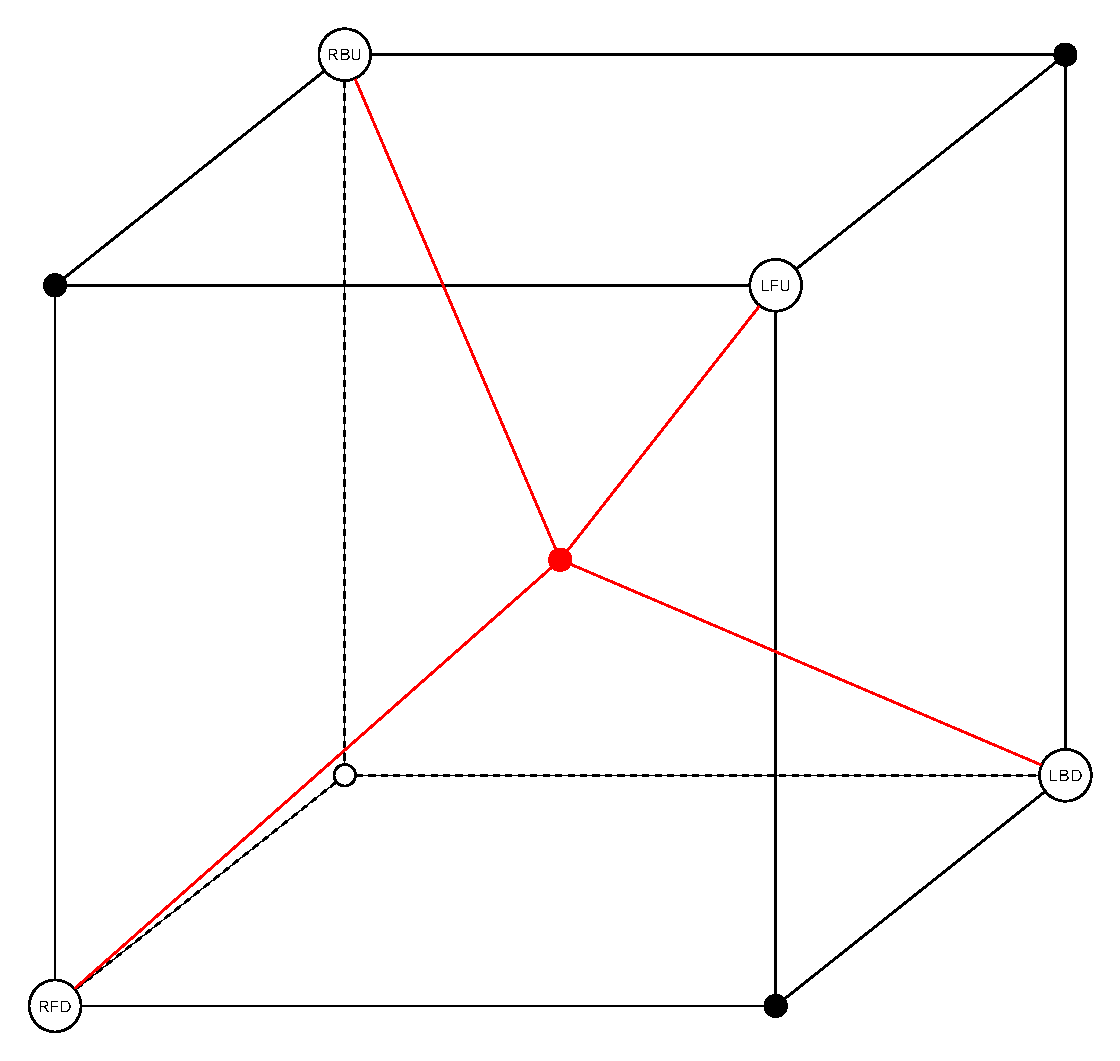
\includegraphics[width=.45\columnwidth]{tetrarec-cube}} \quad
\subfloat[Spazio Tetraedrico]
{\label{fig:tetracube}%
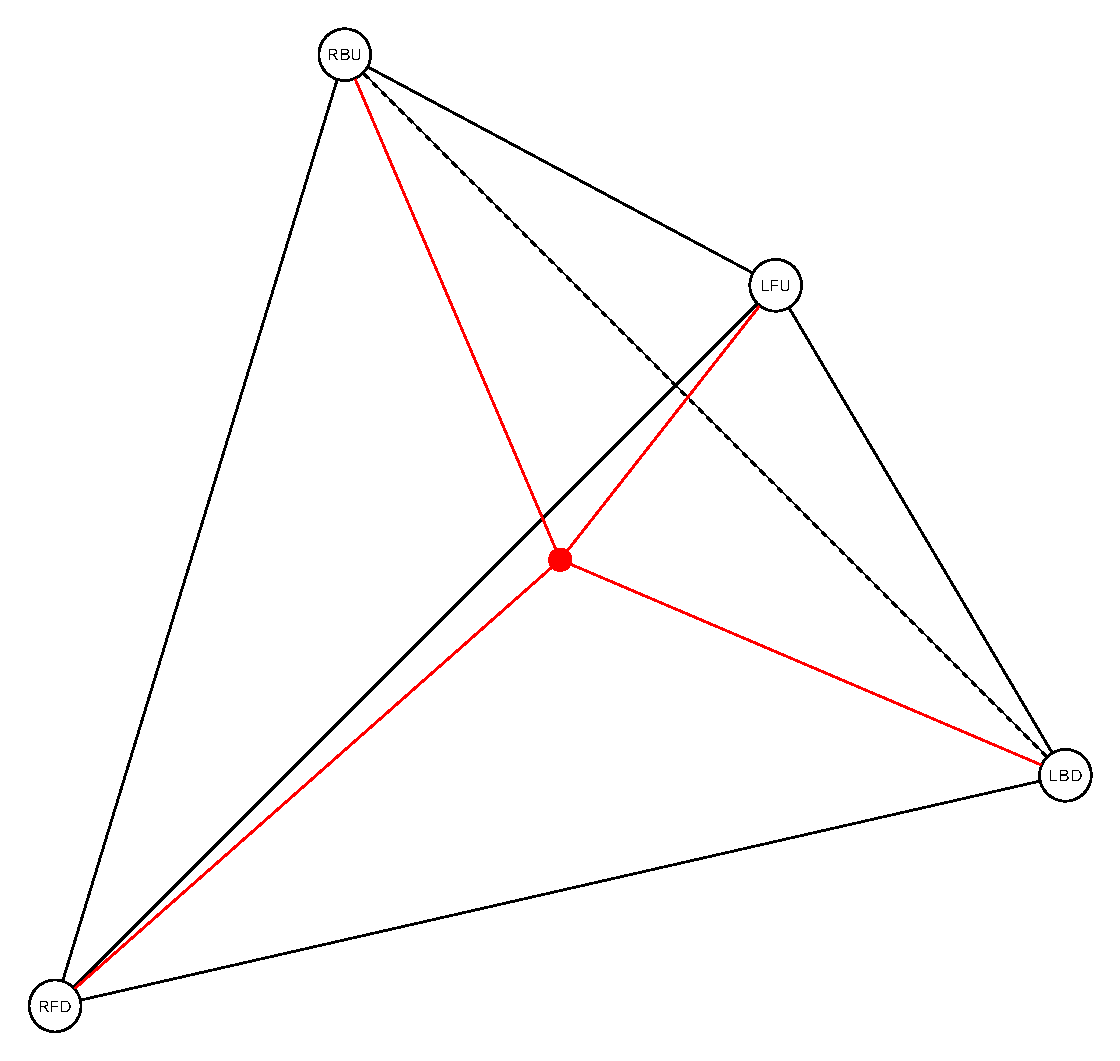
\includegraphics[width=.45\columnwidth]{tetrarec-tetrahedron}} \\
\caption[Spazio Tetraedrico]{Spazio Tetraedrico}
\label{fig:tetratetra}
\end{figure}

%5 parole ancora su Gerzon e ambisonic

La tecnologia descritta da Gerzon permette di descrivere un complesso sonoro
tridimensionale mediante armoniche sferiche denominato \emph{B-Format},
generato da una matrice di scomposizione dei quattro segnali del \emph{A-Format}.
Il \emph{B-Format}, composto da un'armonica di ordine \emph{zero} denominata $ W $
e tre vettori direzionali del \emph{primo} ordine denominati $ X, Y, Z $ può descrivere
vettori spaziali in tutte le dierezioni dello spazio sonoro.

Per la descrizione dello spazio sonoro di \emph{appunti} è stato utilizzato il
sistema di diffusione omnidirezionale \emph{S.T.ONE} in grado di riprodurre direttamente
segnali \emph{A-Format}.

Tracciare questa cartografia acustica della chiesa, tramite risposta all'impulso,
ha portato all'uso di 4 sweep esponeziali, dove agli angoli di un quadrato è
stato disposto il microfono soundfield. La scelta di forma è congiunta alla
disposizione di quattro altoparlanti tetraedrici nella sala da concerto, dove
lo strumentista si colloca tra i due altoparlanti anteriori.
La misurazione  tramite \emph{sweep esponenziale} è stata implementata su software
\emph{Pure Data}. Il segnale di chirop è stato riprodotto mediante altoparlante
tetraedrico \emph{S.T.ONE} e registrato attaverso il microfono \emph{SoundField SPS200}.

\begin{figure}
\centering
{\includegraphics[width=.95\columnwidth]{dolor}}
\caption[Pianta S. Luca]{Pianta S. Luca}
\label{fig:tetratetra}
\end{figure}

%************************************************
\section*{Struttura}
\label{sec:struttura}
%************************************************

Costruzione dell'environment


Tutto in ppppp l'idea  è di ricordanza dei suoni più che dell'effettivo sguardo “concreto”.

Fare i due schemi

Sono partito da due voci che instaurano un rapporto intervallare intorno alla sesta minore.

Questo rapporto intervallare modula sempre in corrispondenza di un centro
(della seconda voce) che è il sib. Mentre  la prima voce segue un processo poco
più complesso: mette in gioco la qualità dei battimenti.

(generati sia dallo spazio tramite convoluzione sia dal sassofono).
La qualità del battimento è fondamentale e questa trasformazione entro la seconda
minore è sia gioco intorno al polo in quell'istante sia “interruttore” per
lo spostamento del polo.

\begin{figure}
\centering
{\includegraphics[width=.95\columnwidth]{dolor}}
\caption[Appunti Partitura]{Appunti Partitura}
\label{fig:tetratetra}
\end{figure}

1)Struttura formale iniziale (astratta):
Anche qui la struttura la divido in 7 parti ma il discorso è sempre duale (A/B),
tra suoni tenuti fino alla perdita di forma e suono che costruisce un senso di fraseggio.
A= zona informale, corone
B=Voce, volontà di fraseggio

in realtà questa scelta di discendenza non viene praticata correttamente.
Ho seguito la mia esperienza per arrivare ad un fine: non rendere subito questa
idea di spostamento delle componenti frequenziali verso il basso.

1)Struttura iniziale (astratta):
Struttura è divisa in 7 blocchi ma il discorso è sempre duale (A/B), tra suoni
tenuti fino alla perdita di forma e suono che costruisce un senso di fraseggio.

A= zona informale, corone
B=Voce, volontà di fraseggio

Tutto in ppppp l'idea  è di ricordanza dei suoni più che dell'effettivo sguardo “concreto”.
Per semplificare invece il discorso riverbero della chiesa, quello che avviene è
uno stazionamento di determinate frequenze che tramite i feedback che costituiscono
il riverbero aumentano di ampiezza. L'aumento di ampiezza corrisponde anche ad un loro
decadimento più lento e questo determina anche la scelta delle frequenze successive a
quella in risonanza con la chiesa: questo per arrivare  battimento/modulazionie di
ampiezza data dalla stanza stessa (quasi un squarcio del riverbero)

%
% \subsection{Mane}
% \lipsum[2]
%
% \subsection{Tekel}
% \lipsum[3]
%
% \subsection{Fares}
% \lipsum[4-5]

%% !TEX encoding = UTF-8
% !TEX TS-program = pdflatex
% !TEX root = ../Tesi.tex
% !TEX spellcheck = it-IT

%************************************************
\chapter{Ipsum}
\label{cap:ipsum}
%************************************************

\lipsum[1]

\section{Lorem}
\lipsum[2]

\section{Ipsum}
\lipsum[3]

\section{Dolor}
\lipsum[4-5]
\appendix
% !TEX encoding = UTF-8
% !TEX TS-program = pdflatex
% !TEX root = ../Articolo.tex
% !TEX spellcheck = it-IT

%************************************************
\section{Dolor}
\label{sec:dolor}
%************************************************

\lipsum[1]

\subsection{Mane}
\lipsum[2]

\subsection{Tekel}
\lipsum[3]

\subsection{Fares}
\lipsum[4-5]

% *****************************************************************
% Materiale finale
%******************************************************************
% !TEX encoding = UTF-8
% !TEX TS-program = pdflatex
% !TEX root = ../CME-III-ARTICOLO.tex
% !TEX spellcheck = it-IT

%*******************************************************
% Bibliografia
%*******************************************************
\nocite{*}
\printbibliography
% !TEX encoding = UTF-8
% !TEX TS-program = pdflatex
% !TEX root = ../Tesi.tex
% !TEX spellcheck = it-IT

%*******************************************************
% Dichiarazione
%*******************************************************
\cleardoublepage
\phantomsection
\pdfbookmark{Dichiarazione}{Dichiarazione}
\chapter*{Dichiarazione}
\thispagestyle{empty}

Lorem ipsum dolor sit amet, consectetuer adipiscing elit. Ut purus elit, vestibulum ut, placerat ac, adipiscing vitae, felis. Curabitur dictum gravida mauris. Nam arcu libero, nonummy eget, consectetuer id, vulputate a, magna. Donec vehicula augue eu neque.

Pellentesque habitant morbi tristique senectus et netus et malesuada fames ac turpis egestas. Mauris ut leo. Cras viverra metus rhoncus sem. Nulla et lectus vestibulum urna fringilla ultrices.

\bigskip
 
\noindent\textit{\myLocation, \MakeTextLowercase{\myTime}}

\smallskip

\begin{flushright}
    \begin{tabular}{m{5cm}}
        \\ \hline
        \centering\myName \\
    \end{tabular}
\end{flushright}

\end{document}